\documentclass[cjk]{beamer}  
\usepackage{xeCJK}  
\usepackage{mathdots}  
\usepackage{graphicx}  
\usepackage{float}  
\usepackage{multirow}  
\usepackage{amsfonts, amsmath, mathrsfs, amsbsy, amssymb, dsfont,setspace}
%\usetheme{Warsaw}  
\usetheme{CambridgeUS}
\begin{document} 
\title{基于压缩感知的多径环境下室内动目标定位}  
  \author{黄臣}  
  \date{\today}  
  \frame{\titlepage}  
  \begin{frame}
	\frametitle{Background}
	穿墙雷达成像是现在的研究热点,在城市反恐、灾害救援等方面都起到了较为重要的
	作用。在室内环境下的雷达成像中,往往不能忽视的是多径的干扰,以及墙内部的
	反射等带来的虚像。此外,为了重建高分辨率的图像,使用常规
	方法如反向投影(BP)往往需要采集和处理大量的
	数据。
	\par 针对上述问题的考虑,本文提出一种基于压缩感知的方法,以解决在
	已知建筑物
	几何结构的情况下,多径环境下的目标检测和速度估计。
  \end{frame}
  \begin{frame}
	\frametitle{Signal Model}
	我们设发射的信号为持续时间为$T_p$的调制宽带脉冲:$\Re\{s(t)\exp(j2\pi f_{c}t)\}$
	其中$t$为快时间(fast time),$s(t)$为复基带上的脉冲。
	\par $K$个宽带脉冲由各发射机以
	$T_r$的脉冲重复间隔(PRI)来传输。每个脉冲引索$k=0,\ldots, K-1$代表慢时间(slow time)。
	\par 在有$P$点目标、$M$个发射机的场景下时,第$k$个脉冲的第$p$个目标的位置为:
	\begin{equation}
	 \boldsymbol x_{p}(k)=(x_{p}+v_{xp}kMT_{r}, y_{p}+v_{yp}kMT_{r})
	\end{equation}
  \end{frame}
  \begin{frame}
	\frametitle{Signal Model}
	在第$n$个接收器上,收到的第$p$个目标反射的由第$m$个发射机所发射的第$k$个
	脉冲可以被表示为:
	\begin{equation}
	  \begin{split}
	  z_{mnk}^{p}(t)=&\sigma_{p}s\left(t-kMT_{r}-mT_{r}-\tau_{pmn}(k)\right)\\
	  &\times\exp\left(-j2\pi f_{c}\left(kMT_{r}+mT_{r}+\tau_{pmn}(k)\right)\right)
	  \end{split}
	\end{equation}
	其中$\sigma_{p}$为第$p$个目标的反射率,$\tau_{pmn}(k)$为双基双向时延。
	我们对目标空间进行尺寸为$N_{x}\times N_{y}$的网格离散化,目标速度也进行
	同样的离散化,这样就能得到$N_{x}N_{y}N_{v}\times 1$的状态矩阵$\boldsymbol\sigma$。
	需要注意的是,网格的分辨率直接影响了稀疏重建的计算复杂度以及对目标速度和
	位置估计的精确度。
  \end{frame}
  \begin{frame}
	\frametitle{Signal Model}
	我们将收到的信号$z_{mnk}(t)$进行采样间隔为$T_s$的$T$次均匀采样,得到长度为$T\times 1$的向量${\boldsymbol z}_{mnk}$,此时式(2)被表示为:
	\begin{equation}
	  {\boldsymbol z}_{mnk}={\boldsymbol\Psi}_{mnk}{\boldsymbol\sigma}
	\end{equation}
	其中${\boldsymbol\Psi}_{mnk}$为字典矩阵:
	\begin{equation*}
	  \begin{split}
	  {[{\boldsymbol\Psi}_{mnk}]}_{i, p}=&\, s\left(t_{i}-kMT_{r}-mT_{r}-\tau_{pmn}(k)\right)\\
	  &\times\exp\left(-j2\pi f_{c}\left(kMT_{r}+mT_{r}+\tau_{pmn}(k)\right)\right),\\
	  &i=0,\ldots, T-1,\quad p=0,\ldots, N_{x}N_{y}N_{v}-1.
	  \end{split}
	\end{equation*}
  \end{frame}
  \begin{frame}
	\frametitle{Signal Model}
	除了感兴趣的目标反射的回波外,内墙壁和外墙面与空气交接处反射的无关回波,
	以及两个墙壁组成的墙角反射的回波,都分别建模如下:
	\begin{equation}
	  \begin{split}
	  z_{kmn}^{\rm wall}(t)=\sum_{b=0}^{N_{\rm w}-1}\sigma_{b}^{\rm wall}&s\left(t-kMT_{r}-mT_{r}-\tau_{bmn}^{\rm wall}\right)\\
	  &\times\exp\left(-j2\pi f_{c}\left(kMT_{r}+mT_{r}+\tau_{bmn}^{\rm wall}\right)\right)
	  \end{split}
	\end{equation}
	\begin{equation}
	  \begin{split}
z_{kmn}^{\rm corner}(t)=\sum_{u=0}^{N_{\rm c}-1}\sigma_{umn}^{\rm corner}&s\left(t-kMT_{r}-mT_{r}-\tau_{umn}^{\rm corner}\right)\\
  &\times\exp\left(-j2\pi f_{c}\left(kMT_{r}+mT_{r}+\tau_{umn}^{\rm corner}\right)\right)
	  \end{split}
	\end{equation}
  \end{frame}
  \begin{frame}
	\frametitle{Signal Model}
	第$u$个墙角的反射率取决于第$m$个发射机和第$n$个接收机的位置,计算公式为:
	\begin{equation}
	  \begin{split}
	  \sigma_{umn}^{\rm corner}& =\left({j2\sqrt{\pi}\over\lambda}\right)^{1\over 2}2L_{u}\\
	 &\quad\times{\rm sinc}\left[{4\pi L_{u}\over\lambda}\left(\cos\left(\psi_{um}^{\rm t}-\tilde{\psi}_{u}\right)-\cos\left(\psi_{un}^{\rm r}-\tilde{\psi}_{u}\right)\right)\right]\\
	 &\quad\times\!\!\left\{ \begin{array}{ll}\sin\!\left({\psi_{um}^{\rm t}+\psi_{un}^{\rm r}-2\tilde{\psi}_{u}\over 2}\right)\!, & \psi_{un}^{\rm r},\psi_{um}^{\rm t}\!\in\!\!\left[\tilde{\psi}_{u},\tilde{\psi}_{u}+{\pi\over 4}\right]\\
	  \cos\!\left({\psi_{um}^{\rm t}+\psi_{un}^{\rm r}-2\tilde{\psi}_{u}\over 2}\right)\!, & \psi_{un}^{\rm r},\psi_{um}^{\rm t}\!\in\!\!\left[\tilde{\psi}_{u}\!+\!{\pi\over 4},\tilde{\psi}_{u}\!+\!{\pi\over 2}\right]
	\end{array} \right.
	  \end{split}
	\end{equation}
	其中$\tilde{\psi}_{u}$为第$u$个墙角的方位角,$\psi_{um}^{\rm t},\psi_{un}^{\rm r}$为入射角和反射角。
  \end{frame}
  \begin{frame}
	\frametitle{Signal Model}
	穿墙雷达成像主要依靠反向投影或延迟求和的波束形成(DSBF),由于
	直接叠加以慢时间$k$为引索的图像值,会让动目标变得模糊,所以这里考虑引入
	目标速度的线性模型。从而可以得到对$K$个脉冲的总和在第$p$个格点上的图像
	值的计算式:
	\begin{equation}
	  \begin{split}
	  I_{p}\!=\!{1\over KMN}\sum_{k=0}^{K-1}\sum_{m=0}^{M-1}\sum_{n=0}^{N-1}&z_{mnk}\big(t+\tau_{pmn}(k)  \big)\ast s^{\ast}(-t)\vert _{t=0},\\
	  & p=0, 1,\ldots, N_{x}N_{y}N_{v}-1 
	  \end{split}
	\end{equation}
	其中$s^{\ast}(-t)$为匹配滤波器的冲激响应。
  \end{frame}
  \begin{frame}
	\frametitle{Multipath Propagation}
	式(3)建立的模型没有考虑到引入多径,在此我们将重点讨论多径传播模型。多径可能
	发生在内壁,地板和天花板的表面。由于使用窄仰角波束宽度的天线时,来自于
	地板和天花板的多径回波往往非常弱,所以我们只需要考虑来自内壁的多径回波。
	其中内壁的反射可分为下面几种情况:
	\par 1.一阶多径,即在发射机到目标反射回接收机的整个传播过程中,只在内壁上
	发生一次反射。这种情况在多径传播中占主要部分。
	\par 2.二阶多径,即往返路径上经历了两次二次反射,又可在细分为两次反射都发生
	在同一内壁上的准单基情况,和分别发生在两面内壁上的双基情况。
	\par 3.更高阶的多径情况,即发生更多次的二次反射,这里不予考虑。
  \end{frame}
  \begin{frame}
	\frametitle{Multipath Propagation}
	内墙的多径反射,我们可以通过使用虚目标的概念来描述其传输路径。如下图所示,
	在计算第$m$个发射机活动时,接收机$n$和目标$p$之间的单向传播延迟$\tau_{pmn}^{({\cal P}^{\prime})}$,我们可以等价交换为计算延迟$\tau_{pmn}^{(\tilde{\cal P}^{\prime})}$。
	在不考虑前墙时,延迟只需通过用两端的欧氏距离除以传播速度即可,若是考虑
	前墙的折射,通过斯涅尔定律即可计算。
	\begin{figure}
	  \centering
	  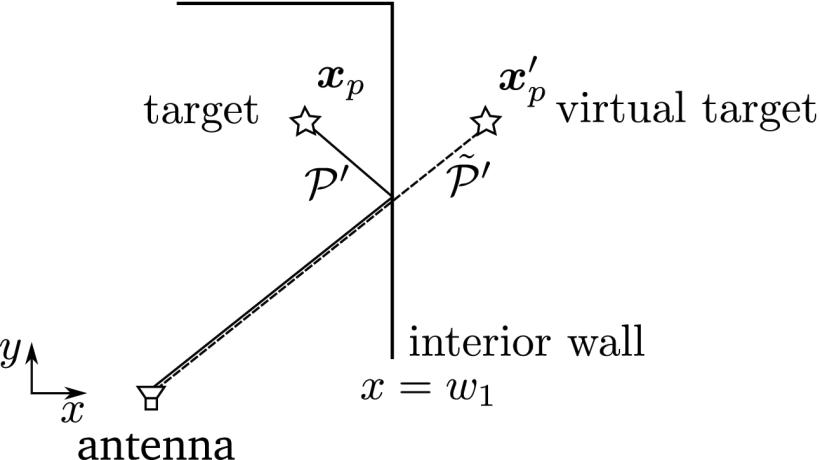
\includegraphics[width=0.5\textwidth]{fig1.jpg}
%	  \caption{虚目标传播示意图}
	\end{figure}
  \end{frame}
  \begin{frame}
	\frametitle{Multipath Propagation}
	从发射端到接收端的传播路径,共有以下9种情况,其中第$r$条路径的复振幅记为
	$\Gamma_{pmn}^{(r)}$,由于直接往返的路径复振幅$\Gamma_{p}^{(0)}$最强,所以我们对所有的$\Gamma_{p}^{(r)}$进行归一化处理,
	$g_{p}^{(r)}$为第$r$条路径对应的权值。
	\begin{equation}
	  g_{p}^{(r)}={\Gamma_{p}^{(r)}\over\Gamma_{p}^{(0)}},\quad r=0,\ldots, R-1,\quad p=0,\ldots, N_{x}N_{y}N_{v}-1
	\end{equation}
	\begin{figure}
	  \centering
	  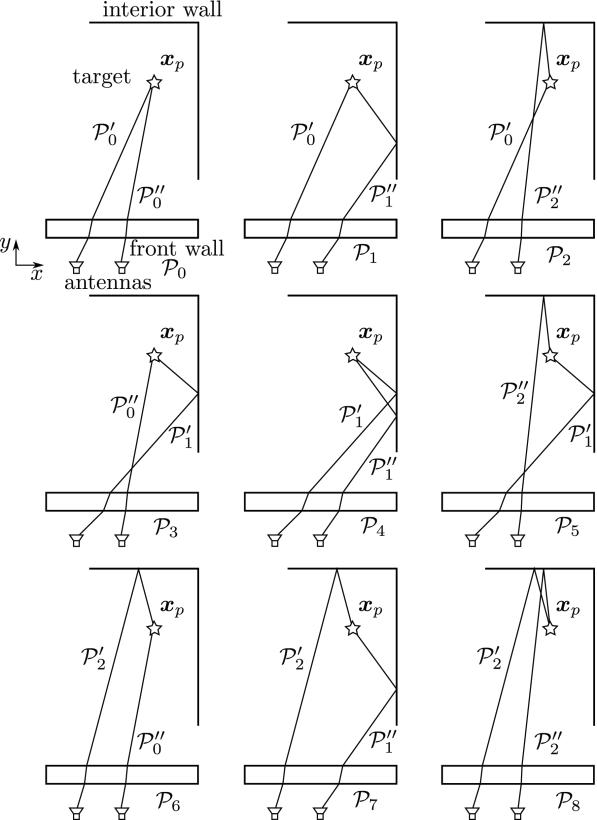
\includegraphics[width=0.25\textwidth]{fig2.jpg}
	\end{figure}
  \end{frame}
  \begin{frame}
	\frametitle{Multipath Propagation}
	多径情况下,各条传播路径的延迟和加权对应的接收信号可表示为:
	\begin{equation*}
	  {\boldsymbol z}={\boldsymbol\Psi}^{(0)}{\boldsymbol\sigma}^{(0)}+{\boldsymbol G}^{(1)}{\boldsymbol\Psi}^{(1)}\bar{\boldsymbol\sigma}^{(1)}+\cdots+{\boldsymbol\Psi}^{(R-1)}{\boldsymbol G}^{(R-1)}\bar{\boldsymbol\sigma}^{(R-1)}
	\end{equation*}
	${\boldsymbol G}^{(r)}={\rm diag}(g_{0}^{(r)}, g_{1}^{(r)},\ldots, g_{N_{x}N_{y}N_{v}-1}^{(r)})$为路径权值矩阵,字典${\boldsymbol\Psi}^{(r)}$与(3)式定义方式相似。令${\boldsymbol\sigma}^{(r)}={\boldsymbol G}^{(r)}\bar{\boldsymbol\sigma}^{(r)}$,上式
	可改写为:
	\begin{equation}
	 {\boldsymbol z}={\boldsymbol\Psi}^{(0)}{\boldsymbol\sigma}^{(0)}+{\boldsymbol\Psi}^{(1)}{\boldsymbol\sigma}^{(1)}+\cdots+{\boldsymbol\Psi}^{(R-1)}{\boldsymbol\sigma}^{(R-1)} 
	\end{equation}
  \end{frame}
  \begin{frame}
	\frametitle{Multipath Propagation}
	我们希望从收到的多径回波中估计出目标的运动速度,在不同的传播路径中目标具有
	不同的视在多普勒速度。在双基雷达模型中,以发射机和接收机为焦点的零多普勒
	速度轨迹形成的椭圆的法线即为可观察速度分量。参考前面描述传输路径引入虚目标
	的方法,这里我们同样引入虚发射/接收机,来分析视在多普勒速度。
	\begin{figure}
	  \centering
	  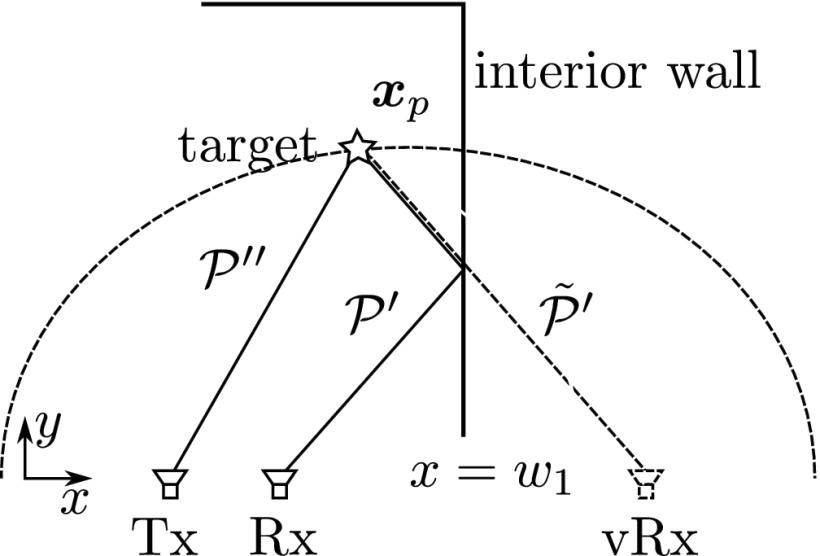
\includegraphics[width=0.4\textwidth]{fig3.jpg}
	\end{figure}
  \end{frame}
  \begin{frame}
	\frametitle{Multipath Propagation}
	视在多普勒速度可以用传播延迟来计算:
	\begin{equation}
	  v_{D, pmn}^{(r)}={1\over K-1}\sum_{k=0}^{K-2}c{\tau_{pmn}^{(r)}(k+1)-\tau_{pmn}^{(r)}(k)\over T_{r}}
	\end{equation}
	在天线阵列足够小时,视在多普勒速度主要取决于传播路径和目标位置。
  \end{frame}
  \begin{frame}
	\frametitle{Compressive Sensing Based Scene Reconstruction}
	从快时间,慢时间或者是发射/接收机四个方面来进行回波欠采样时,都可以体现
	出压缩感知的好处。式(9)可以稀疏表示为:
	\begin{equation}
	  \bar{\boldsymbol z}={\boldsymbol{\Phi z}}={\boldsymbol\Phi}\left({\boldsymbol\Psi}^{(0)}{\boldsymbol\sigma}^{(0)}+{\boldsymbol\Psi}^{(1)}{\boldsymbol\sigma}^{(1)}+\cdots+{\boldsymbol\Psi}^{(R-1)}{\boldsymbol\sigma}^{(R-1)}\right)
	\end{equation}
	其中${\boldsymbol\Phi}\in\mathbb{R}^{J\times TMNK}$为测量矩阵,$J$为减少测量的数量。
	\begin{equation*}
	  \begin{split}
	  {\boldsymbol\Phi}=\left({\boldsymbol\Phi}_{1}\otimes{\boldsymbol I}_{N_{\rm d}K_{\rm d}T_{\rm d}}\right)&\cdot\left({\boldsymbol\Phi}_{2}\otimes{\boldsymbol I}_{MK_{\rm d}T_{\rm d}}\right)\cdot\left({\boldsymbol\Phi}_{3}\otimes{\boldsymbol I}_{MNT_{\rm d}}\right)\\
	  &\cdot{\rm diag}\left({\boldsymbol\Phi}_{4}^{(0)},\ldots,{\boldsymbol\Phi}_{4}^{(MNK-1)}\right)
	  \end{split}
	\end{equation*}
  \end{frame}
  \begin{frame}
	\frametitle{Compressive Sensing Based Scene Reconstruction}
	在式(11)中,我们已知测量值$\bar{\boldsymbol z}$,希望通过稀疏重建来恢复
	目标状态信息$\tilde{\boldsymbol\sigma}$,考虑到多径的影响,我们可以利用
	目标状态向量表现出的组稀疏结构,将问题转化为解决混合$\ell_{2}/\ell_{1}$
	范数最小化问题来实现组稀疏重构未知向量${\boldsymbol\sigma}$:
	\begin{equation}
	 \hat{\boldsymbol\sigma}=\arg\min_{\tilde{\boldsymbol\sigma}}{1\over 2}\Vert\bar{\boldsymbol z}-{\boldsymbol\Phi}\tilde{\boldsymbol\Psi}\tilde{\boldsymbol\sigma}\Vert_{2}^{2}+\mu\Vert\tilde{\boldsymbol\sigma}\Vert_{1, 2} 
	\end{equation}
  凸优化问题可以使用SparSA算法或块正交匹配追踪(BOMP)算法进行求解。
	其中$\mu$为正则化参数,正则项为:
	\begin{equation*}
	 \Vert\tilde{\boldsymbol\sigma}\Vert_{1, 2}=\sum_{p=0}^{N_{x}N_{y}N_{v}-1}\left\Vert\left[\sigma_{p}^{(0)},\sigma_{p}^{(1)},\ldots,\sigma_{p}^{(R-1)}\right]^{T}\right\Vert_{2} 
	\end{equation*}
  \end{frame}
  \begin{frame}
	\frametitle{Compressive Sensing Based Scene Reconstruction}
  考虑到稀疏重建算法算法复杂度大的问题,这里提出一种两步重建的方法:首先通过
  压缩感知来估计目标位置,随后使用传统多普勒方法估计目标速度。因此相对于求解
  式(12),这里只需要重建目标的空间信息即可,即测量矩阵$\breve{\boldsymbol\Phi}\in\mathbb{R}^{T_{\rm d}M_{\rm d}N_{\rm d}\times TMN}$在慢时间域不进行采样。
  \begin{equation}
	\begin{split}
	\hat{\boldsymbol\sigma}^{(r)}(k)&\!=\!\arg\min_{{\boldsymbol\sigma}^{(r)}(k), r=0,\ldots, R-1}{1\over 2} \left\Vert\breve{\boldsymbol z}(k)\!-\!\!\sum_{r=0}^{R-1}\breve{\boldsymbol\Phi}\breve{\boldsymbol\Psi}^{(r)}{\boldsymbol\sigma}^{(r)}(k)\right\Vert_{2}^{2}\\
	&+\mu\sum_{p=0}^{N_{x}N_{y}-1}\left\Vert\left[\sigma_{p}^{(0)}(k),\sigma_{p}^{(1)}(k),\ldots,\sigma_{p}^{(R-1)}(k)\right]^{T}\right\Vert_{2}
  \end{split}
  \end{equation}
  \end{frame}
  \begin{frame}
	\frametitle{Compressive Sensing Based Scene Reconstruction}
  第二步进行速度的估计,仅选择有振幅的目标$N_p$,将有目标的区域的状态值用${\boldsymbol b}_{p}^{(r)}=[\hat{\sigma}_{p}^{(r)}(0),\ldots,\hat{\sigma}_{p}^{(r)}(K-1)]^{T}\in{{\rm C}{\hskip-5pt}{\rm I}}^{K}$
  表示。对${\boldsymbol b}_{p}^{(r)}$进行离散时间傅里叶变换得到$B_{p}^{(r)}(\omega)$,其峰值为视在多普勒速度。
  \begin{equation}
	v_{D, p}^{(r)}={c\over\pi f_{c}}\arg\max_{\omega}B_{p}^{(r)}(\omega)
  \end{equation}
  \end{frame}
  \begin{frame}
	\frametitle{Results}
	\begin{figure}
	  \centering
	  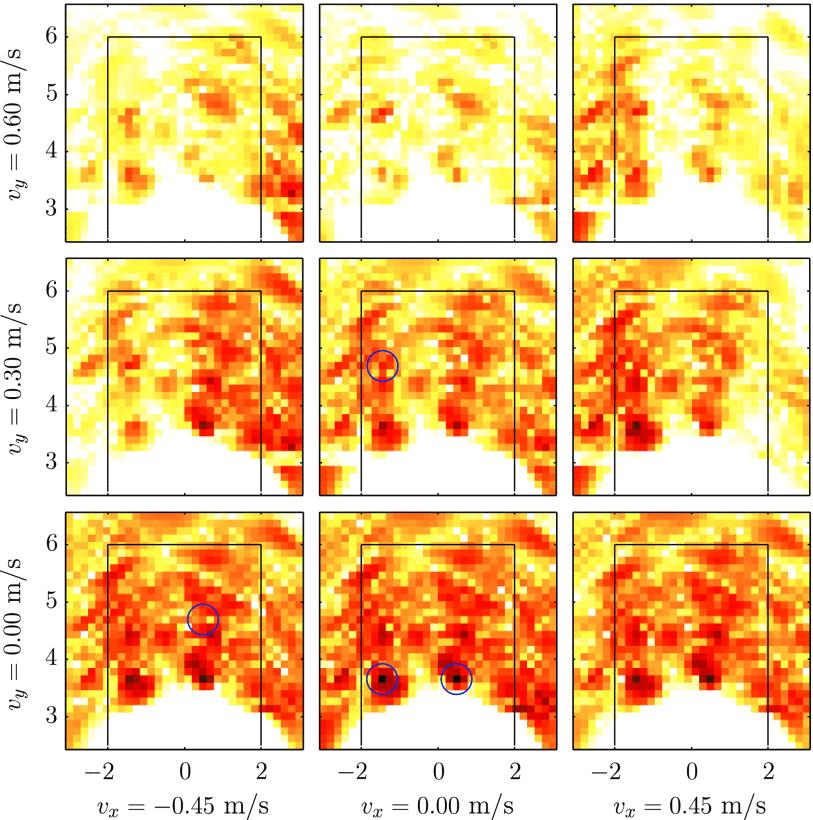
\includegraphics[width=0.4\textwidth]{fig4.jpg}
	\end{figure}
	上图为延迟求和波束形成的仿真结果,我们共设置了四个目标:两个静目标(0.5, 3.7)m,(−1.5, 3.7)m;两个动目标(0.5, 4.7)m,(−1.5, 4.7)m,速度为:(−0.45, 0)m/s和(0, 0.3)m/s。 
  \end{frame}
  \begin{frame}
	\frametitle{Results}
	\begin{figure}
	  \centering
	  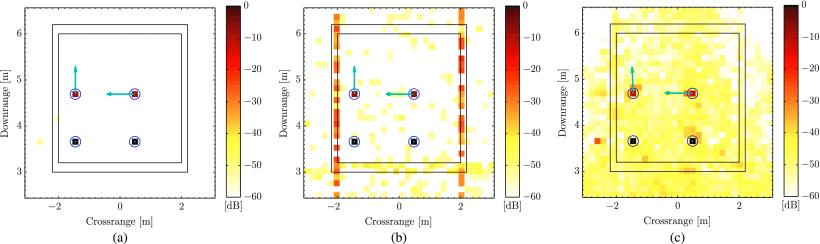
\includegraphics[width=0.9\textwidth]{fig5.jpg}
	\end{figure}
  \end{frame}
  \begin{frame}
	\frametitle{Results}
	\begin{figure}
	  \centering
	  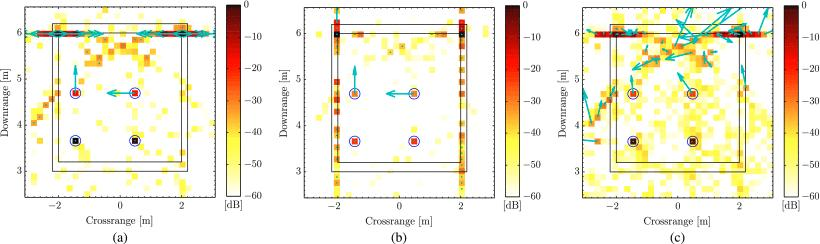
\includegraphics[width=0.9\textwidth]{fig6.jpg}
	\end{figure}
  \end{frame}
\end{document}
  \begin{frame}
	\frametitle{Compressive Sensing Based Scene Reconstruction}
  \end{frame}
  \begin{frame}
	\frametitle{Compressive Sensing Based Scene Reconstruction}
  \end{frame}
  \begin{frame}
	\frametitle{Compressive Sensing Based Scene Reconstruction}
  \end{frame}
  \begin{frame}
	\frametitle{Compressive Sensing Based Scene Reconstruction}
  \end{frame}
	\begin{figure}[H]
	  \centering
	  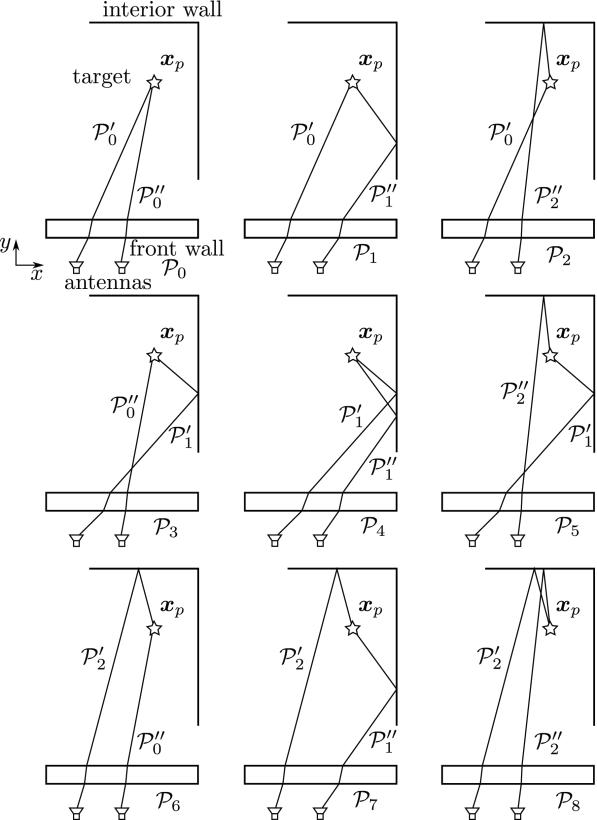
\includegraphics[width=0.5\textwidth]{fig2}
	  \caption{CSI处理流程图}
	\end{figure}
